\documentclass[conference,11pt]{IEEEtran}
\IEEEoverridecommandlockouts
\usepackage[verbose,expansion=alltext,stretch=50]{microtype}
\usepackage{graphicx}
\usepackage{booktabs}
\usepackage[hidelinks]{hyperref}
\usepackage[ruled,vlined]{algorithm2e}
\usepackage{xcolor}
\usepackage{float}
\usepackage{subcaption}
\usepackage[labelformat=parens,labelsep=quad,skip=3pt]{caption}

\newcommand{\link}[1]{{\color{blue}\href{#1}{#1}}}
\title{Exploring A* Search For Single and Multi Layer Routing}

\author{
\IEEEauthorblockN{Mohamed Shawky}
\IEEEauthorblockA{Computer Engineering\\
Cairo University\\
Email: mohamed.sabae99@eng-st.cu.edu.eg} \\
\IEEEauthorblockN{Remonda Talaat}
\IEEEauthorblockA{Computer Engineering\\
Cairo University\\
Email: Remonda.Bastawres99@eng-st.cu.edu.eg}
\and
\IEEEauthorblockN{Mahmoud Adas}
\IEEEauthorblockA{Computer Engineering\\
Cairo University\\
Email: mahmoud.ibrahim97@eng-st.cu.edu.eg} \\
\IEEEauthorblockN{Evram Youssef}
\IEEEauthorblockA{Computer Engineering\\
Cairo University\\
Email: evram.narouz00@eng-st.cu.edu.eg}
}

\begin{document}
\maketitle

\begin{abstract}

\end{abstract}

\begin{IEEEkeywords}

\end{IEEEkeywords}

\section{Introduction}
Fast running systems requires many transistors, which makes the manufacturing process very hard.
Many Chips have millions or even billions of transistors which affects the circuit timing, power consumption, chip reliability and manufacturability that complicate all the design rules.
One of the most important challenge is routing to connect the transistors, without causing any problem on the chip.
Routing problem, in \emph{VLSI}, is considered an \emph{NP-hard} problem, so it is divided into two design phases, \emph{global routing} where the grid is constructed with its nodes and edges,
and \emph{detailed phase} (our target) to find shortest paths to connect the required pins in the grid together.
Many algorithms can be used to solve routing problem, as it can be formulated as grid search problem, where speedup and optimality are a trade-off.
We try \emph{Lee's}, \emph{Mikami-Tabuchi}, \emph{Steiner tree} and \emph{A* search} algorithms, where our main approach was A* search.
We compare the different algorithms based on their execution time and length of metal.



We discussed the Detailed Routing problem, and shows that it can be formulated as gird search problem.
A* algorithm with euclidean distance as cost function was our main approach in the problem solution.
We tried different gird search techniques and compared their results with our main approach with respect to performance and time, and found that
A* achieves the better performance in some cases and same performance in the others in acceptable time compared to other algorithms.

\section{Terminology}
\subsection{Basics} %There's a space here, don't erase it.
\begin{itemize}
	\item Maze: it's a $[D,W,H]$ matrix that contains cells, used to simulate the grid.
    \item D: number of layers, W: width of the layer, H: height of the layer.
    \item Cells: each cell is a pin, a cell could represent a pin or an obstalce.
	\item Pin: the part where transistors gets connected to.
	\item Source: the starting point (pin) that needs to be connected to some targets.
	\item Tatgets: one or many point/s (pin/s) that need to be connected to the source in minimum cost.
	\item Obstacle: a block that wires can't go through.
	\item Vias: like a ladder to the upper or lower layer.
	\item Wire: what connects the pins with each others.
	\item Path: the route which the wire will take in order to connect the source with all of the targets.
	\item Cost: the length of the path, the longer the wire the larger the delay.
	\item Multi-layers: instead of having only one $2D$ grid, we have multiple grids, stacked vertically.
	\item Steiner Point: intermediate points that targets can be connected to.
\end{itemize}

\subsection{Assumptions} 
\begin{itemize}
    \item All wires are the same size.
    \item No geometric rules violations(ie. spacing).
    \item All pins are placed at the center of cells.
\end{itemize}

\label{terminologySection}

\section{Related Work}
\subsection{Basic History}
    In 1959, Moore, Edward F. presented one of the first shortest path through a maze algorithm
    \cite{MooreRef}, after a couple of years in 1961 Lee, C. Y. presented the idea of simulating the 
    board wiring on electronics board as a Maze \cite{LeeRef}. Starting from there the idea of Lee Maze
    has been revisited many times, in 1983 Hightower, D. made more contribution to the idea such that
    using modern computers and virtual memories we can memic the routing problem precisely providing 
    different techniques \cite{HightowerRef}.

\subsection{Router Problem Anatomy}
    The Routing problem has many sections and subsections, in this paper we are mainly concerned with
    Detailed routing. Detailed routing is divided into many subsections, as you can see in fig.\ref{fig:routing_anat} 
    and we are exploring Maze and Line Search subsections.

    \begin{figure}[H]
        \centering
        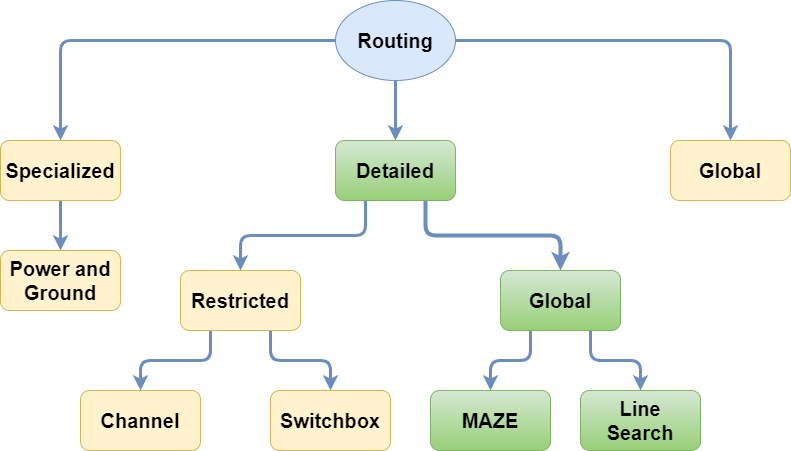
\includegraphics[width=0.4\textwidth]{figures/routing_anatomy.png}
        \caption{Anatomy of various routing techniques.}
        \label{fig:routing_anat}
    \end{figure}

    In the next section we are showing how various algorithms work, and discussing three 
    algorithms, first the \nameref{LeeSection} it's a Maze based algorithm, second the 
    \nameref{MikamiSection} it's a Line-Probe algorithm, and finally the \nameref{SteinerSection} 
    it's a baseline algorithm.

\subsection{Simulation environment}
    Rapidly we'll describe our Simulation's properties:
    \begin{itemize}
        \item Detailed routing (not global)
        \item System is presented as $3D$ Grid,$[D, W, H]$
        \begin{itemize}
            \item D: number of layers 
            \item W: width of each grid
            \item H: height of each grid
        \end{itemize}
        \item Only one source exist as a start.
        \item Multiple targets exist (nested), fan-out.          
        \item Consistent Cost: no bending cost, no extra cost due to vias.
        \item Vias cost is $1$.
        \item Within the same 2D grid path could be horizontally or/and vertically
            chosen.
    \end{itemize}

\subsection{Explored Techniques}
    Before diving into these algorithms make sure to read the \nameref{terminologySection} section first.
    \newline

    \subsubsection{Lee algorithm}
    \label{LeeSection}
    This is one of the most common and origin routing algorithms \cite{LeeRef}.

    If there's a path between source $S$ and some target $T$, the algorithm will definitely find it,
    and in case of consistent cost (ie. no variable cost) the algorithm will not only find the 
    a path but also the shortest one.

    It uses BFS (breadth-first search) to connect targets with the source.

    It works appropriately with multiple layers (ie, where vias exist).

    The algorithm has three main stages:
    \begin{itemize}
        \item Expansion
        \item Back-tracking
        \item Clean up
    \end{itemize}

    The \textit{Expansion} stage fig.\ref{expansionStage} creates like a \textit{halo} shape around the source,
    and it gets larger and the cost of each cell is incremented,
    unless there's an obstacle (block cell),
    until it hits a target and terminates,
    if the expansion reached it's limit with no target hit, this means that the target/s is/are not
    reachable.
% TODO: since the [H] forces the graph to be placed after that section
% extra spacing occur
% so when you are finished with everything..make sure it looks good
    \begin{figure}[H]
        \label{fig:expansionStage}
        \centering

        \begin{subfigure}[b]{0.3\linewidth}
            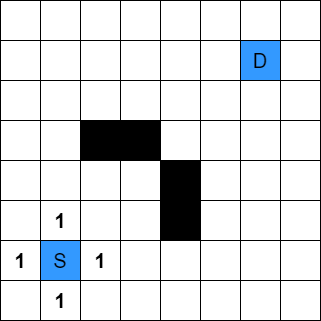
\includegraphics[width=\linewidth]{figures/Lee Stages/grid.png}
            \caption{itr 1}
        \end{subfigure}
        \begin{subfigure}[b]{0.3\linewidth}
            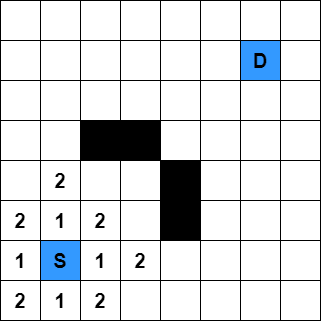
\includegraphics[width=\linewidth]{figures/Lee Stages/grid 1.png}
            \caption{itr 2}
        \end{subfigure}
        \begin{subfigure}[b]{0.3\linewidth}
            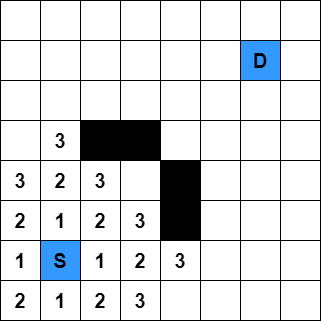
\includegraphics[width=\linewidth]{figures/Lee Stages/grid 2.png}
            \caption{itr 3}
        \end{subfigure}
        \begin{subfigure}[b]{0.3\linewidth}
            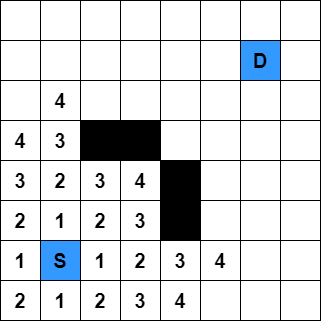
\includegraphics[width=\linewidth]{figures/Lee Stages/grid 3.png}
            \caption{itr 4}
        \end{subfigure}
        \begin{subfigure}[b]{0.3\linewidth}
            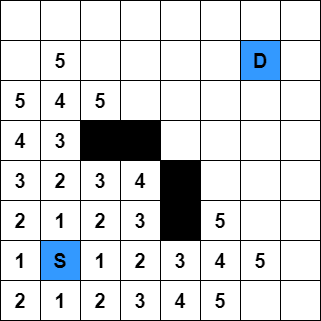
\includegraphics[width=\linewidth]{figures/Lee Stages/grid 4.png}
            \caption{itr 5}
        \end{subfigure}
        \begin{subfigure}[b]{0.3\linewidth}
            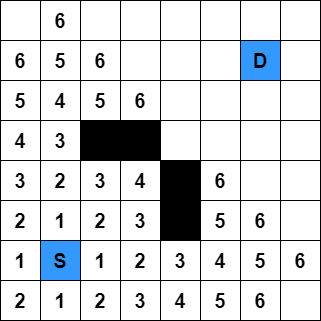
\includegraphics[width=\linewidth]{figures/Lee Stages/grid 5.png}
            \caption{itr 6}
        \end{subfigure}
        \begin{subfigure}[b]{0.3\linewidth}
            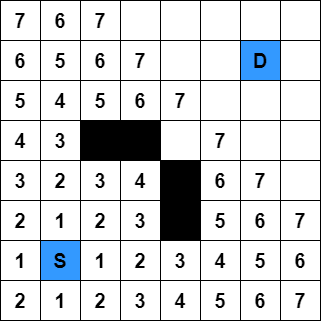
\includegraphics[width=\linewidth]{figures/Lee Stages/grid 6.png}
            \caption{itr 7}
        \end{subfigure}
        \begin{subfigure}[b]{0.3\linewidth}
            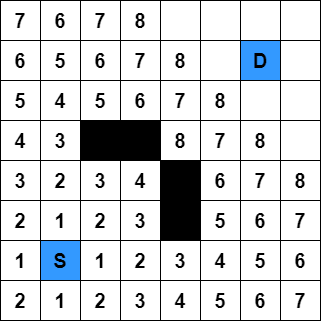
\includegraphics[width=\linewidth]{figures/Lee Stages/grid 7.png}
            \caption{itr 8}
        \end{subfigure}
        \begin{subfigure}[b]{0.3\linewidth}
            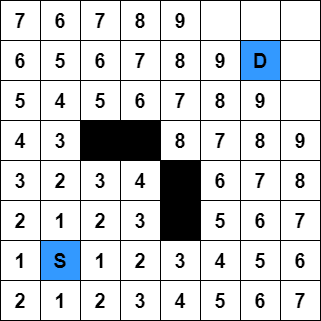
\includegraphics[width=\linewidth]{figures/Lee Stages/grid 8.png}
            \caption{itr 9}
        \end{subfigure}
        \begin{subfigure}[b]{0.3\linewidth}
            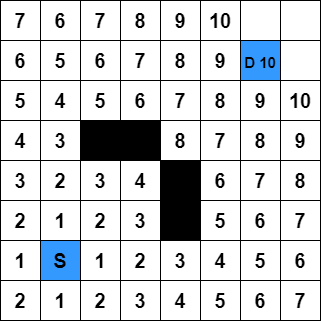
\includegraphics[width=\linewidth]{figures/Lee Stages/grid 9.png}
            \caption{itr 10}
        \end{subfigure}
        
        \caption{Expansion Stage}
      \end{figure}
      

    The \textit{Back-tracking} stage fig.\ref{fig:backtrackingStage} gets the path from the target $T$
    to the source $S$.
    Since we are dealing with consistent cost, then the backtracking stage is not that much of an issue
    all we have to do is to decrement the cost by $1$ from the target, until we reach the source.
    In other versions where inconsistent cost exist, and the cost of the path is the total length of it.
    \textbf{Data structure} such as \textbf{priority queue} is used to \textit{pop-up}
    the cell with minimum cost.

    \begin{figure}[H]
        \centering
        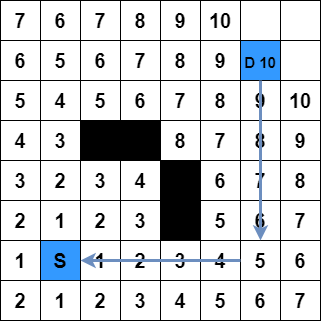
\includegraphics[width=0.35\textwidth]{figures/Lee Stages/back-track.png}
        \caption{Back-tracking Stage}
        \label{fig:backtrackingStage}
    \end{figure}

    The \textit{Clean up} stage fig.\ref{fig:cleanUpStage} converts the path from the source
    to the target into obstacles (blocks) so that no interference between pathes may exist.
    and then starts to connect another target to the source with that path of obstacles added.

    \begin{figure}[H]
        \centering
        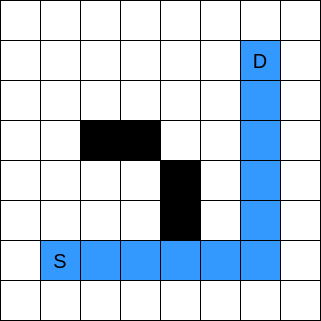
\includegraphics[width=0.35\textwidth]{figures/Lee Stages/clean_up.png}
        \caption{Clean up Stage}
        \label{fig:cleanUpStage}
    \end{figure}

    \subsubsection{Mikami-Tabuchi algorithm}
    \label{MikamiSection}

    \subsubsection{Steiner algorithm}
    \label{SteinerSection}
    is the baseline algorithm for our work.

    The definition Steiner Tree is very general, we are mainly concerned with menimum Stiener tree problem,
    and it's algorithm.

    Minimum Steiner Tree $(MST)$ algorithm provides the minimum spanning tree that may exist in the graph.

    It's basic idea is that, after including the first path -the shortest/closest target to the source-
    any other target that will be connected to the source may be connected to any point of the 
    earlier extracted path.

    The algorithm works as follows \cite{SteinerRef}:
    \newline
    %TODO: when finished, adjust this
    \begin{algorithm}[]
        \SetAlgoLined
        \KwResult{Optimal/Minimum path between source and all target cells.}
        Find the closest target to the source\;
        \While{$T$ Doesn't span all terminals}{
        Select terminal $x$ not in $T$ that is closest to a vertex in $T$\;
        Add to $T$ the shortest path that connects $x$ with $T$\;
        }
         \caption{Steiner Tree algorithm For Maze Routing}
    \end{algorithm}
        
    As mentioned before, Steiner always provide the optimal path -when it exists-,
    but the Steiner Tree problem is $NP$ Hard problem, both exact and approximate solutions exist,
    and as for our condition we are interested in the exact solution.

    The solution provided to the problem is very simple, the minimum path ot be found 
    every time is provided using $Dijkstra$ algorithm, due to all this computations as the dimensions of the graph get larger and the number
    of targets increase the time complexity increases exponentially.

    The intermediate points that are now sources and targets can be connected to are called
    Steiner Points.



\section{Methodology}
\subsection{Motivation}
Metal routing is a critical step in systems integration process, where each source is connected to its fan-outs using non-crossing metal. Routing in a modern chip, with millions or even billions of transistors, can be very complicated and cumbersome, so the manufacture process has moved to automatic routing. 

Automatic routing is a very vast field, with several techniques being developed through time. Automatic routing involves lots of problems like finding shortest non-blocked path and VIAs in multi-layer routing. 

Automatic routing techniques are always a trade-off between optimality and speed. Some techniques target execution time by reaching a sub-optimal solution. Others target optimal solution with very high execution time.

In this work, we seek a good balance between performance and optimality of solution by introducing the usage of A* search for automatic routing with a modified cost function.

\subsection{Formulation}
\begin{figure}
    \centering
    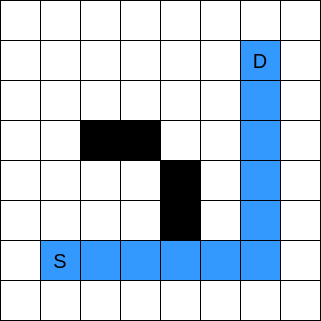
\includegraphics[width=0.4\textwidth]{figures/grid.png}
    \caption{Example of occupancy grid map (OGM), where S is the source, D is the destination, white cells aren't occupied, black cells are occupied and blue cells represent the path.}
    \label{fig:grid}
\end{figure}

Routing is formulated as a grid search problem \ref{fig:grid}, where an occupancy grid map \emph{(OGM)} is provided with some source and destination cells to be joined. The \emph{OGM} cells can have the value of $1$ for occupied cell or $0$ for empty cell. The \emph{OGM} can be of multiple levels, in case of multi-layer routing, where the cell can have a third value to indicate that the cell can be used as a VIA. Only 4-neighbor cells are considered, so the path can move up, down, left or right. The path can also move from one level to another through VIA cells.

Given this problem formulation, several grid search and shortest path algorithms can be used to find the optimal path between each source and its given destinations. These algorithms can vary based on optimality and performance.

The two main metrics considered in this work are path length and execution time. Total length of metal, covering the grid, is used as a measure of solution optimality. It's defined as the number of grid cells, on which the metal is placed for routing.

Execution time is used as a measure of algorithm performance. It's simply the total elapsed time by the algorithm to find all required paths.

To develop a comparison framework between the baselines and our proposed technique, we propose the following assumptions:
\begin{itemize}
    \item All wires are of the same size.
    \item No geometric rules violation (i.e. spacing).
    \item All pins are placed at the center of cells.
\end{itemize}

\subsection{Baseline}
To measure the validity and performance of our proposed method, three main baselines are used. These baselines are well-established algorithms that are currently used in industry.

\subsubsection{Maze Routing (Lee's Algorithm)}
The first baseline algorithm, to be considered, is \emph{maze routing}, discussed in \ref{LeeSection}. Maze routing is one of the most well-established and widely-used algorithms in metal routing. It consists of a wide range of algorithms and techniques. \emph{Lee's algorithm} is the basic maze routing solution and it's considered as our first baseline for comparison. This algorithm is basically a grid search algorithm for routing.

\subsubsection{Mikami-Tabuchi’s Algorithm}
The second considered baseline algorithm is \emph{Mikami-Tabuchi’s} algorithm, discussed in \ref{MikamiSection}. Unlike \emph{Lee's algorithm}, this algorithm is a line search technique that adopts line-search operations. It can find a path between source and destination cells, but it doesn't guarantee the shortest possible path.   

\subsubsection{Steiner Tree Algorithm}
\emph{Steiner tree} spans though the given subset of vertices in a given graph. Steiner tree, discussed in \ref{SteinerSection}, is suitable for any situation, where the task is minimize cost of connection among some important locations, like VLSI Design, Computer Networks, etc. So, Steiner tree is considered as our final baseline algorithm.

\subsection{Modified A* Search}
\begin{figure}
    \centering
    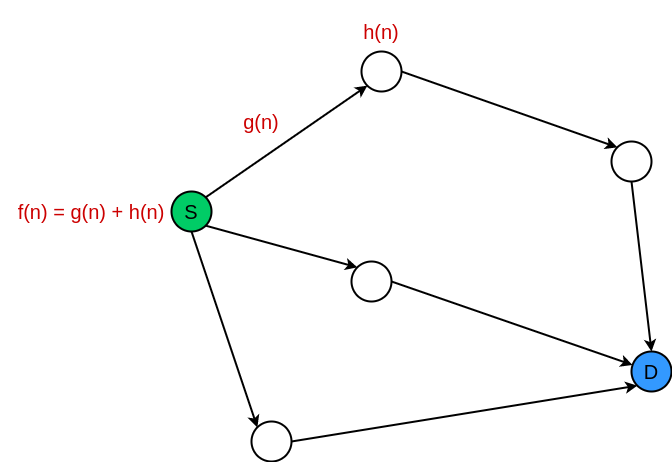
\includegraphics[width=0.4\textwidth]{figures/a_star.png}
    \caption{An illustrative example for A* search process and cost function.}
    \label{fig:astar}
\end{figure}

The main contribution of this work is the usage of \emph{A* search}, with modified cost function, as a new routing technique. The main idea of \emph{A* search}, as shown in fig.\ref{fig:astar}, is the usage of some heuristic function to assign a cost for each node. To define a path from a source node to a destination node, the nodes that minimizes the estimated path cost are chosen at each step. The main objective is to minimize the following function:

\begin{equation} \label{eq:astar}
f(n) = g(n) + h(n)
\end{equation}
Where \emph{f(n)} is the total cost of the path from a specific node, \emph{g(n)} is the cost of the edge between current node and next chosen node and \emph{h(n)} is the estimated cost of the next chosen node based on the used heuristic function.

Thus, the required information to solve an \emph{A* search} problem is the cost of edge between each two nodes and the heuristic function to get an estimated cost for each node.

\begin{figure}
    \centering
    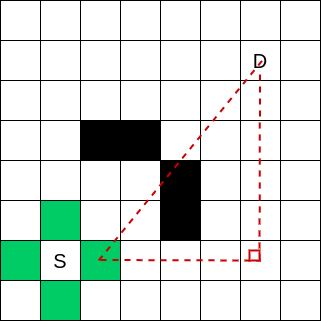
\includegraphics[width=0.4\textwidth]{figures/grid_euclid.png}
    \caption{An illustrative example for the new heuristic function based on Euclidean distance. The distance is measured between the centres (pins) of both cells.}
    \label{fig:euclid}
\end{figure}

The \emph{OGM} representation of the routing problem can be formulated to become an \emph{A* search} problem. The edge cost \emph{g(n)} is always $1$, as the path can only move from one cell to an adjacent cell. The heuristic function, proposed in this work, is \emph{Euclidean distance} between next chosen cell and destination cell, as shown in  fig.\ref{fig:euclid}. So, the cost of taking any of the adjacent cells is \emph{Euclidean distance} $+$ $1$, which can be simplified to \emph{Euclidean distance} between an adjacent cell and destination cell.\\

The proposed algorithm can be summarized as follows:

\begin{algorithm}
\SetAlgoLined
\KwResult{Optimal path between source and destination cells.}
 append source cell to the path\;
 \While{destination not reached}{
  get adjacent cell that minimizes euclidean distance\;
  append cell to the path\;
  \If{current cell is blocked}{
   remove current cell from path\;
   backtrack to the previous cell\;
   continue\;
   }
 }
 \caption{Modified A* Search For Automatic Routing}
\end{algorithm}


\section{Experimental Results}
\subsection{Goals}
We want to answer those questions about our proposed algorithm:
\begin{enumerate}
    \item How fast is it?
    \item How short are the found paths?
\end{enumerate}
Because \textit{fast} and \textit{short} are relative terms. We need to calculate them in a comparison with other approaches. 
We chose to compare our results against:
\begin{itemize}
    \item Mikami: known by its speed, but very far from the optimal answer. Would give us insights on how much speed we have achieved.
    \item Steiner Tree: Finds the optimal answer. We will use it to know whether our results are optimal.
    \item Lee Maze: First algorithm used in the industry. Helps us know how far we have progressed relative to the industry practical techniques.
\end{itemize}

\subsection{Code}
We implemented our proposed algorithm in \texttt{mod\_a\_star.py}, 
lee maze algorithm in \texttt{maze\_lee.py},
mikami-tabuchi algorithm in \texttt{mikami\_tabuchi.py}
and Steiner tree in \texttt{steiner\_tree.py}.

All scripts read JSON input from the \texttt{stdin} and writes json output to \texttt{stdout}, so we can chain them with the other scripts. And they follow the \texttt{io\_schema.md} specs about io format.

\subsection{IO Specs}
Input contains a $d\times h \times w$ grid matrix, where:
\begin{itemize}
    \item $d \rightarrow$ Number of layers, either 1 or 2.
    \item $h \rightarrow$ Height.
    \item $w \rightarrow$ Width.
\end{itemize}
Each cell is either:
\begin{itemize}
    \item 0 $\rightarrow$ Empty.
    \item 1 $\rightarrow$ Obstacle.
    \item 2 $\rightarrow$ VIA, only when $d=2$ and must exist on the other layer too.
\end{itemize}
Each input contains the source coordinates and a list of targets coordinates.

Output should contain the found paths and their corresponding lengths.

Both input and output should be in JSON format. See \texttt{io\_schema.md} for more details.

\subsection{Helper Scripts}
We wrote a couple of scripts to assist with the comparison and testing:
\begin{itemize}
    \item \texttt{gen-input.py}: Generates random input that follows \texttt{io\_schema.md}. It doesn't guarantee that all targets are reachable. For more info \texttt{\$ python3 gen-input.py --help}
    \item \texttt{verify.py}: Takes the input to the algorithm and its output and verifies the correctness of the result. See \texttt{\$ python3 verify.py --help}
    \item \texttt{random\_test}: Generates infinite random inputs, run given algorithm on each test, and verify the results.
    \item \texttt{random\_comp}: Generates $N$ random input, run each algorithm on each input, calls \texttt{calc\_total.py} to calculate total cost and verify the results.
    \item \texttt{nConst}: Calls \texttt{random\_comp} $M$ times, each time with same number of targets, varying the grid area (w,h).
    \item \texttt{areaConst}: Calls \texttt{random\_comp} $M$ times, each time with same width and height of the input grid, varying the number of targets.
    \item \texttt{merge\_comp}: Merges the outputs of \texttt{random\_comp} into one \texttt{tmp/summary.json} with the summary of the experiment.
    \item \texttt{plot.py}: Plots given \texttt{summary.json} through the stdin to \texttt{tmp/plot}.
\end{itemize}

\subsection{The Experiment}
For simplicity, we assumed all grids are squares. So $w=h$ in all tests.
We also assumed number of layers $d=2$ in all tests.

We need to very the area while the number of targets is constant. And in the other case, vary the number of targets while the area is constant.
And in both, we will record and plot the running times and costs.

We expect some algorithm to take a very big time to calculate the output. Unfortunately we can't just let it run forever. So we just sat the timeout as 5 minutes. This is why we collected the number of found targets, so we compare how many times an implementation has time-outed and resulted in 0 final targets found.

\textbf{Note:} Not all targets in some input have to be reachable. Bigger grids have bigger probability of having non-reachable targets.

We started the experiments by running:
\begin{enumerate}
    \item \texttt{nConst}, which for each area of areas of grid in [10, 15, 20, 50, 100], conducts 5 random experiments on each algo given the same random input (for each experiment) in which the number of targets ($n$) is const and $n = 5$.
    \item \texttt{areaConst}, which for each number of targets in [6, 10, 15, 20, 50], conducts 20 random experiments on each algo given the same random input (for each experiment) in which the area of the grid ($w,h$) is constant and $w = h = 45$.
\end{enumerate}

After running the 2 scripts multiple times and then merging their outputs using \texttt{merge\_comp}, we had so far 396 unique experiment, each experiment is a unique input given to the 4 algorithms and all the 1584 results are in \texttt{summary.json}.

\subsection{Comparisons}
We made the plots using \texttt{plot.py}. The following is the line of thoughts we had through the comparison.

\subsubsection{Running Time Scatter}
We started by scattering all the running time per \#Targets and per Grid Width, see Fig. (\ref{fig:runningTime}). 

The results are not very clear as the points of mikami and lee are compressed down because of Steiner and a*. 

We can also notice a* has some outliers in time, specially in bigger grid widths (50, 100). This is why we may use the median function multiple times instead of the average.

\begin{figure}
\centering

\begin{subfigure}[b]{\linewidth}
    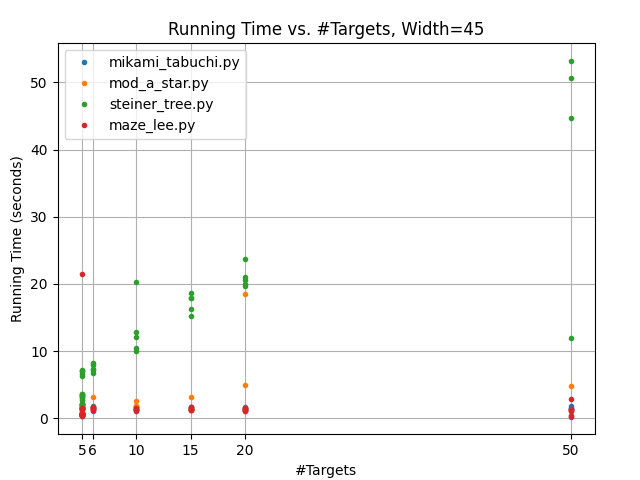
\includegraphics[width=\linewidth]{figures/plots/areaConst.png}
    \caption{Time / \#Targets}
\end{subfigure}
\begin{subfigure}[b]{\linewidth}
    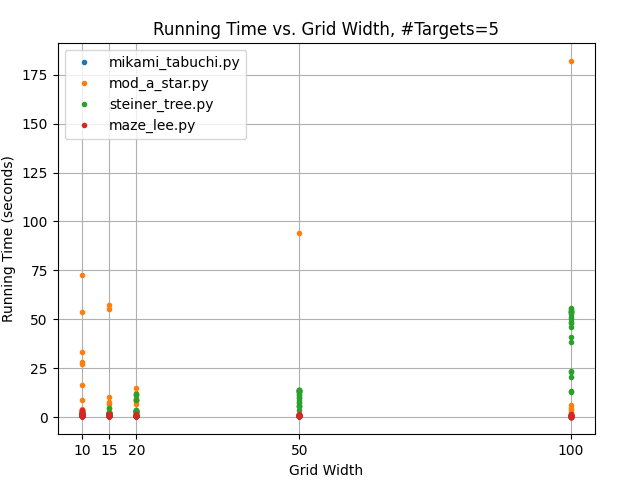
\includegraphics[width=\linewidth]{figures/plots/nConst.png}
    \caption{Time / Grid Width}
\end{subfigure}

\caption{Running Time}
\label{fig:runningTime}
\end{figure}

\subsubsection{Median Running Time}
To make the plots clearer, we calculated the median of the running time instead of scattering all points. See Fig. (\ref{fig:medianRunningTime}).

We notice that both mikami and lee are very fast, they take less than 2 seconds no matter what the input size is.

We also notice that Steiner grows exponentially with both the size of the grid and the number of targets. But it's affected more by the growth of number of targets.

But our new approach grows linearly with only the size of the grid. Its performance is independent from the number of targets.

\begin{figure}
\centering

\begin{subfigure}[b]{\linewidth}
    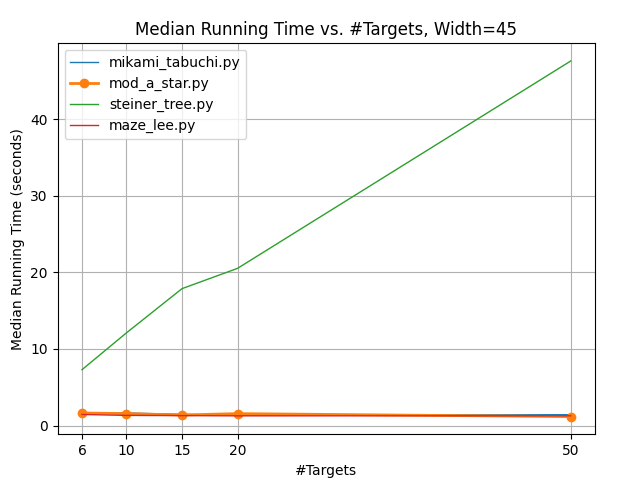
\includegraphics[width=\linewidth]{figures/plots/medianTime_areaConst.png}
    \caption{Median Time / \#Targets}
\end{subfigure}
\begin{subfigure}[b]{\linewidth}
    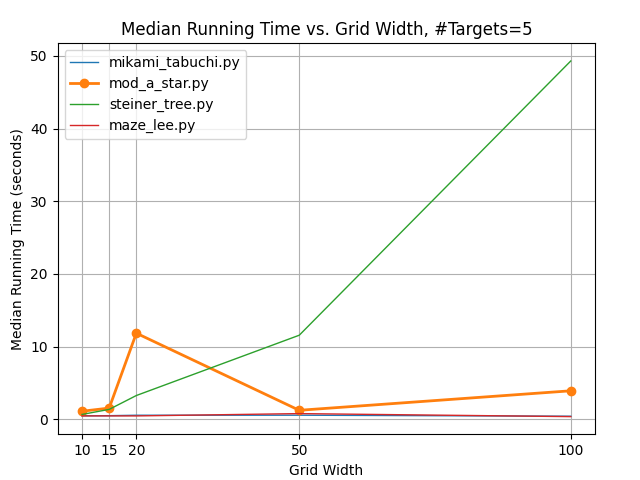
\includegraphics[width=\linewidth]{figures/plots/medianTime_nConst.png}
    \caption{Median Time / Grid Width}
\end{subfigure}

\caption{Median Running Time}
\label{fig:medianRunningTime}
\end{figure}

\subsubsection{Cost}
Next we move on to comparing cost. Fig. (\ref{fig:maxCost}, \ref{fig:avgCost}, \ref{fig:totalCost}) shows maximum, average and total cost respectively achieved by each algorithm per area and per number of targets.

We notice that a* has achieved overall lower costs in the paths it found, regardless of number of targets or grid area. For some reason it didn't find any on $n=50$. 

All algorithms found no results when grid area = 100. Because \texttt{gen-input.py} generated non-reachable points on that size.

Mikami-Tabuchi was the worst overall in the costs.

\begin{figure}
\centering

\begin{subfigure}[b]{\linewidth}
    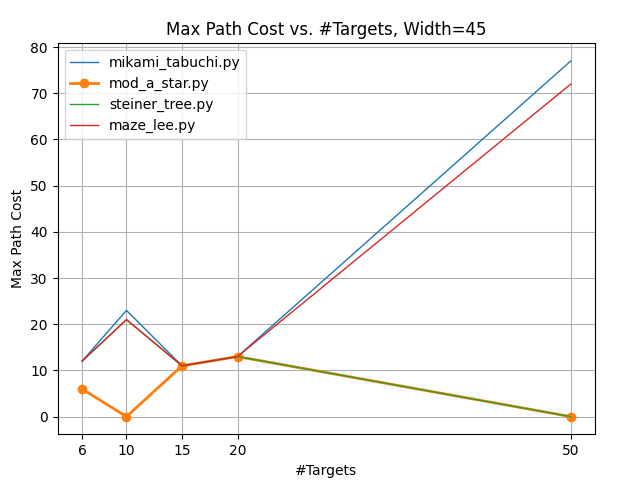
\includegraphics[width=\linewidth]{figures/plots/maxCost_areaConst.png}
    \caption{Max Path Cost / \#Targets}
\end{subfigure}
\begin{subfigure}[b]{\linewidth}
    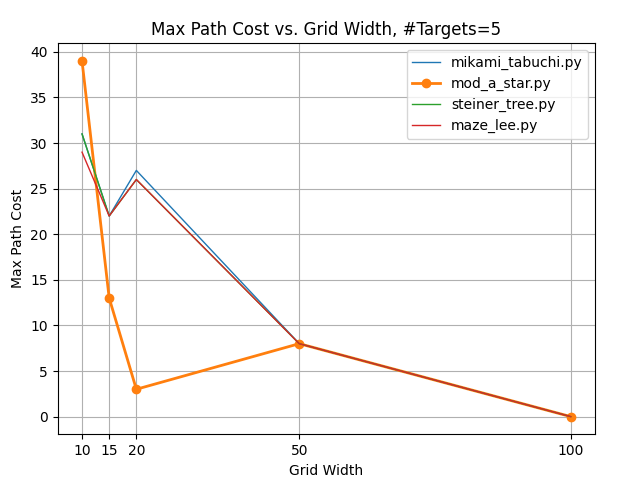
\includegraphics[width=\linewidth]{figures/plots/maxCost_nConst.png}
    \caption{Max Path Cost / Grid Width}
\end{subfigure}

\caption{Maximum Path Cost}
\label{fig:maxCost}
\end{figure}

\begin{figure}
\centering

\begin{subfigure}[b]{\linewidth}
    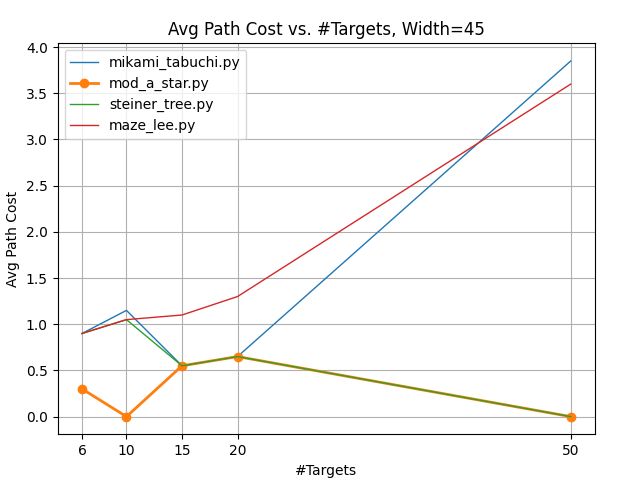
\includegraphics[width=\linewidth]{figures/plots/avgCost_areaConst.png}
    \caption{Avg Path Cost / \#Targets}
\end{subfigure}
\begin{subfigure}[b]{\linewidth}
    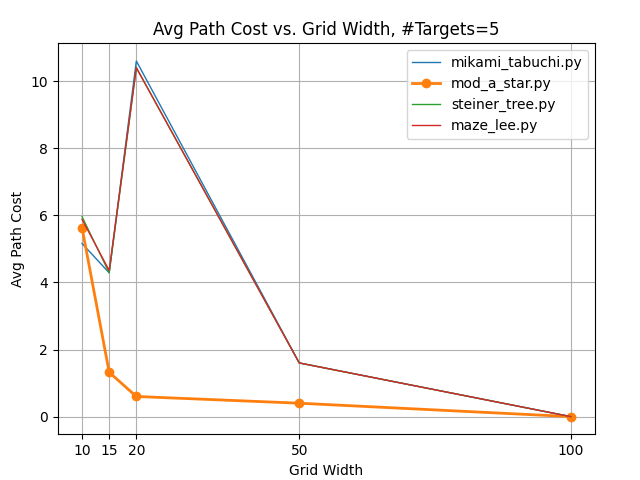
\includegraphics[width=\linewidth]{figures/plots/avgCost_nConst.png}
    \caption{Avg Path Cost / Grid Width}
\end{subfigure}

\caption{Average Path Cost}
\label{fig:avgCost}
\end{figure}

\begin{figure}
\centering

\begin{subfigure}[b]{\linewidth}
    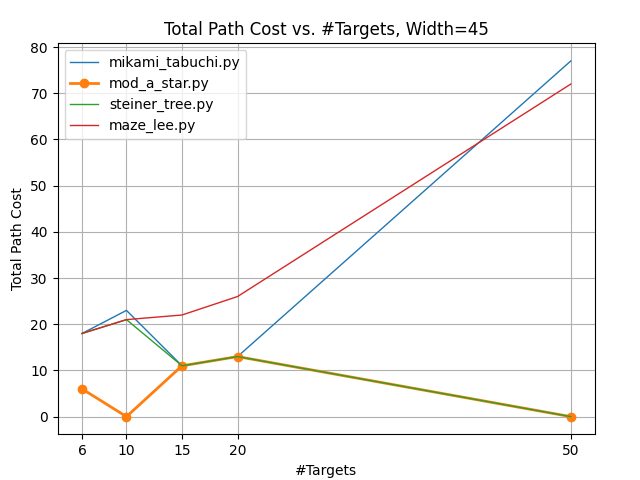
\includegraphics[width=\linewidth]{figures/plots/totalCost_areaConst.png}
    \caption{Total Path Cost / \#Targets}
\end{subfigure}
\begin{subfigure}[b]{\linewidth}
    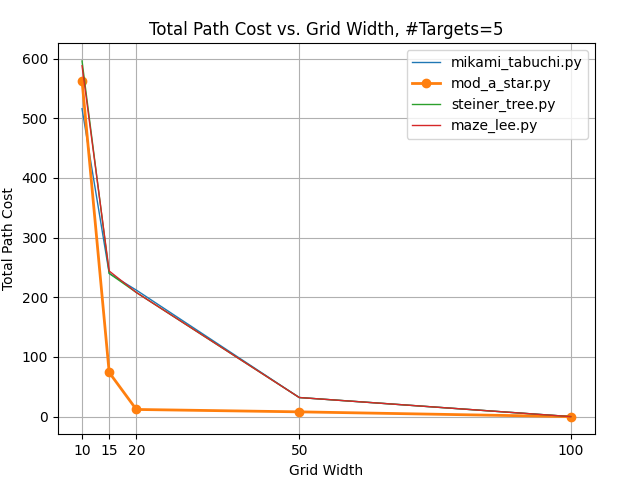
\includegraphics[width=\linewidth]{figures/plots/totalCost_nConst.png}
    \caption{Total Path Cost / Grid Width}
\end{subfigure}

\caption{Total Path Cost}
\label{fig:totalCost}
\end{figure}

\subsubsection{Errors}
We noticed that some algorithms went to 0 on cost. So we calculated the percentage of found targets by each algorithms, to compare how many targets each algorithms found per $n$. Fig. (\ref{fig:percTargets}) shows that percentage.

The percentage of targets alone don't explain the reason why both a* and Steiner had some zero costs.  Is it because of timeouts? Or because some issues with our code?

Fig. (\ref{fig:timeouts}) is a plot of timeouts per area and per $n$. We notice that both Steiner and a* have high time-outing chances compared to Mikami and lee. Unfortunately, we can't increase the timeout threshold more than 5 minutes, otherwise the nearly 2000 tests won't finish executing.

So far, given this data, we can conclude that the high than average error rate of a* and Steiner are due to their high chances of time-outing.

\begin{figure}
\centering
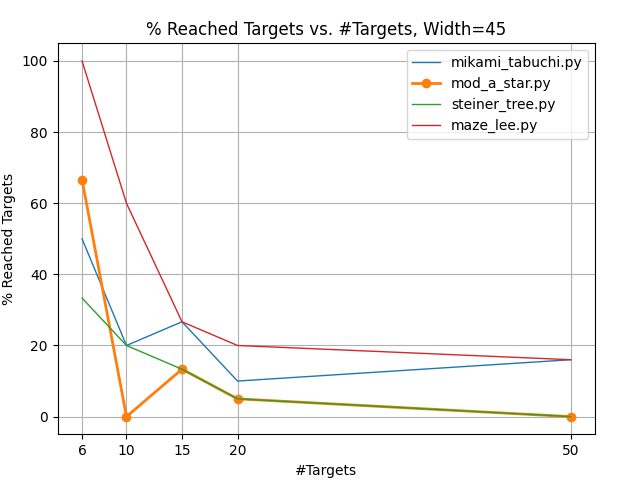
\includegraphics[width=\linewidth]{figures/plots/percTargets_areaConst.png}
\caption{Percentage of Found Targets / \#Targets}
\label{fig:percTargets}
\end{figure}

\begin{figure}
\centering

\begin{subfigure}[b]{\linewidth}
    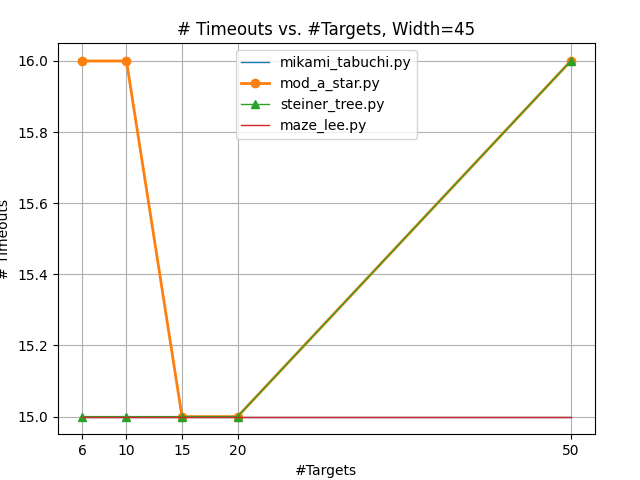
\includegraphics[width=\linewidth]{figures/plots/timeouts_areaConst.png}
    \caption{\#Timeouts / \#Targets}
\end{subfigure}
\begin{subfigure}[b]{\linewidth}
    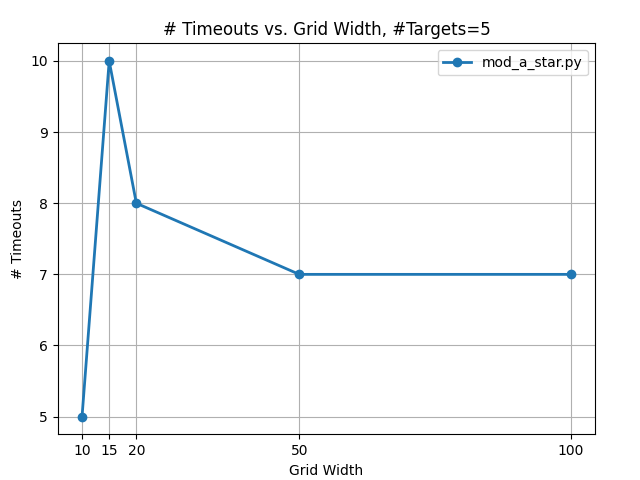
\includegraphics[width=\linewidth]{figures/plots/timeouts_nConst.png}
    \caption{\#Timeouts / Grid Width}
\end{subfigure}

\caption{\#Timeouts}
\label{fig:timeouts}
\end{figure}
    

\section{Conclusion}
In this work, we discuss the \emph{ Detailed Routing } problem, and how it's important challenge in manufacturing process, showing that it can be formulated as gird search problem.
\emph{A* Search} algorithm, with euclidean distance as cost function, is our main approach in the problem solution.
We have tried different gird search techniques and compared their results with our main approach with respect to performance and time, and found that
\emph{A* Search} achieves better performance in some cases and same performance in others, in acceptable time, compared to other algorithms.

\medskip

\bibliographystyle{unsrt}
\bibliography{paper}
    
\end{document}
